\documentclass[11pt]{article}
\usepackage[review]{acl}
\usepackage{times}
\usepackage{latexsym}
\usepackage[T1]{fontenc}
\usepackage[utf8]{inputenc}
\usepackage{microtype}
\usepackage{graphicx}
\usepackage{booktabs}
\usepackage{amsmath}
\usepackage{amssymb}
\usepackage{amsfonts}
\usepackage{array}
\usepackage{xurl}
\usepackage{xcolor}

\title{The Criterion Cannot See What It Does Not Measure: Auditing Capability-Guided Attention Hybridization Against a Named Agent-Commitment Circuit}

\author{Anonymous ACL submission}

\begin{document}
\maketitle
\begin{abstract}
Efficiency-driven model transformations increasingly decide \emph{which internal components to keep} using
causal, capability-guided criteria. HydraHead \citep{tan2026hydrahead} selects which attention heads retain
full attention (FA) versus linear attention (LA) via activation-patching importance on a capability set
$C=\{$long-context retrieval, general ability$\}$. We audit this criterion class against a \emph{named,
causally-verified} agent circuit: the sparse commitment circuit of Qwen3.6-27B (writers h8/h6/h3 at layer
59, opposed by a counter-set), previously shown to carry an agent's decision to commit actions. Computing
HydraHead-style receiver importance for all 384 FA heads, we find retrieval-criticality and
commitment-writing are \emph{anti-aligned}: the commit writers h8/h6 carry zero retrieval criticality
($\kappa{=}0$; stable under doubled probe samples), while the layer's strongest retrieval heads (global
ranks 2 and 4 of the model) are the commitment circuit's \emph{opposers}. Behaviorally, mean-ablating the
capability-non-retained late-band heads collapses task-appropriate commitment --- $P(\text{edit})$ at edit
decision points $0.474{\to}0.167$; emission $0.48{\to}0.18$; the edit/bash differential vanishes
($0.25{\to}0.00$; 18/0 monotonic flips, exact McNemar $p{=}7.6{\times}10^{-6}$) --- worse than \emph{all
five} size-matched random selections (mean $0.33$), because the retrieval-only keep-set is the least
commitment-redundant subset of its size. Restoring just the two named writer heads ($0.5\%$ of FA heads,
identifiable only by causal circuit analysis) recovers baseline exactly (0 flips); keeping two random heads
at identical severity does not ($0.15$--$0.20$ across three seeds vs $0.48$; paired 17/0,
$p{=}1.5{\times}10^{-5}$). Meanwhile the capability
probes that define the criterion register nothing --- and, having failed their positive control, could
not have. Capability-causal $\neq$ safety-causal: transformations should be audited with the circuits one
cares about, because the criterion cannot see what it does not measure --- and neither can its benchmarks.
\end{abstract}

\section{Introduction}

The cost of long-context inference is pushing model builders toward \emph{surgical} efficiency: rather than
compressing uniformly, modern methods identify which components carry the capabilities they care about and
preserve only those. Head-level attention hybridization is the sharpest instance to date: HydraHead
\citep{tan2026hydrahead} keeps full attention (FA) only for heads that are \emph{causally} necessary for
long-context retrieval and general ability --- measured by activation patching with a downstream freeze ---
and converts the rest to linear attention (GDN), matching a 3:1 layer-wise hybrid's long-context
performance at a 7:1 LA-to-FA ratio.

The selection method is sound; it is the same causal toolbox interpretability research uses. The auditable
surface is the \emph{capability set}. A head that is critical for a behavior \emph{outside} $C$ ---
safety, agency, action control --- scores zero and is converted, silently, while every benchmark in $C$
passes. Prior work has shown versions of this blind spot at other granularities and for other objects:
retrieval-oriented head selection drops \emph{reasoning}-critical heads \citep{du2025rlkv}; pruning and
quantization degrade \emph{refusal}-style safety
\citep{wei2024brittleness,patel2025aapp,chen2025qresafe,jahan2025distillation}; compression degrades
agentic \emph{capability} \citep{dong2025acbench}. What has not been done is to take a specific SOTA
selection criterion and causally test, at the granularity of \emph{named individual heads}, whether a
localized \emph{agent-action} circuit survives it.

We can run exactly that audit, because prior work on Qwen3.6-27B located the circuit. In a long-horizon
software agent, the model's decision to commit an action (\texttt{str\_replace\_editor} vs \texttt{bash})
is written by a sparse push--pull circuit in layer 59 (a full-attention layer of the hybrid stack):
writers h8/h6/h3 reproduce the full attention effect ($+0.262 \geq$ all-24 $+0.224$), partially cancelled
by an opposing head set; the writers are induction/copy-style heads reading tool-call history
\citep{vicentino2026lever,vicentino2026brake}. This gives the audit a ground truth most compression
evaluations lack: named heads, causal roles, deterministic decision points, and published baselines.

\paragraph{Contributions.}
(1) A reimplementation of HydraHead's receiver importance on Qwen3.6-27B (384 FA heads, NIAH counterfactual
probes with structure-preserving corruption and downstream-freeze patching), with fidelity gates to the
published commitment-circuit baselines.
(2) \textbf{Anti-alignment}: the commit writers carry zero retrieval criticality ($\kappa{=}0$, stable under
doubled probe samples) and are dropped at any FA budget; the layer's top retrieval heads are the circuit's
opposers (Section~\ref{sec:stage1}).
(3) \textbf{A two-sided causal audit}: under the same ablation, task-appropriate commitment collapses
(monotonic, $p{=}7.6{\times}10^{-6}$) while the criterion's own capability probes register nothing ---
and we show, via a failed positive control, that their ``pass'' is uninformative
(Section~\ref{sec:stage2}).
(4) \textbf{Tight controls}: the capability-guided keep-set is worse for commitment than all five
size-matched random selections; a two-head ``safety term'' (the named writers) restores baseline exactly,
while two random heads at identical severity do not (Section~\ref{sec:stage34}).
(5) An honest accounting of what a pre-registered audit of this kind can and cannot conclude
(Section~\ref{sec:limitations}), extending the interpretability-as-audit program from ``audit the fixed
model'' to \emph{audit the transformation}.

\section{Related work}

\textbf{Head-level hybridization and retrieval heads.} HydraHead \citep{tan2026hydrahead} builds on the
retrieval-head line \citep{wu2024retrieval,xiao2024duo,tang2024razor}: a sparse set of heads carries
precise long-context copying, and efficiency methods can treat the rest cheaply.
\citet{du2025rlkv} show retrieval-based selection has a blind spot for \emph{reasoning}; we show the
analogous --- and behaviorally sharper --- blind spot for an agent's \emph{action-commitment} circuit,
and audit the criterion itself rather than proposing a new one.

\textbf{Compression vs.\ safety.} Safety-relevant structure is sparse and brittle under pruning and
low-rank edits; notably, \citet{wei2024brittleness} already showed at \emph{weight} granularity that a
capability-aware pruning criterion (Wanda) is the best at preserving perplexity and the \emph{worst} at
preserving safety --- our ``worse than random'' result is the head-level, agent-action instance of that
phenomenon, not a new principle. Individual ``safety heads'' causally carry refusal
\citep{zhou2024safetyheads}; refusal circuits under compression have been studied mechanistically
\citep{yao2025refusalcompressed}; alignment-aware pruning \citep{patel2025aapp} and safety-aware KV-cache
retention \citep{anchorskv2026} already \emph{propose} adding safety terms to selection objectives ---
our contribution there is the audit-derived motivation (a named circuit the criterion scores $\kappa{=}0$),
not the proposal itself. Quantization degrades safety \citep{chen2025qresafe}; distillation transfers task
fidelity but not safety \citep{jahan2025distillation}; compression degrades agentic capabilities
\citep{dong2025acbench}; hybrid linear-attention conversion is known to degrade instruction-following at
the benchmark level \citep{yang2025untangling}; and capability-blind compression can look competitive
because aggregate metrics under-report specific damage \citep{cgc2026}. These works measure
refusal/toxicity or aggregate capability, at weight/channel/model granularity. What none of them do is
take a specific transformation's \emph{selection criterion} and causally test, at named-head granularity,
whether a localized \emph{agent-action} circuit survives it --- with a nominal restore as the positive
control. That composition, and the anti-alignment finding it surfaces, is the contribution.

\textbf{Interpretability as audit.} Auditability of MI \emph{experiments} has been argued at the venue
level \citep{makemi2026}, and interpretability-driven model auditing has been articulated as a research
agenda \citep{aigi2026agenda}. We instantiate that agenda against a concrete efficiency transformation:
to our knowledge (and as of this writing no published work cites or audits HydraHead), this is the first
executed circuit-level audit of a head-level FA$\to$LA hybridization criterion.

\section{Method}\label{sec:method}

\textbf{Model and target circuit.} Qwen3.6-27B is a hybrid linear/full-attention stack
(\texttt{full\_attention\_interval}=4): 16 FA layers $\{3,7,\dots,63\}\times 24$ heads $=384$ FA heads
(GQA 24:4, head dim 256, no o\_proj bias). The commitment circuit at L59 --- writers h8/h6/h3, opposers
h16/19/11/4/21/23 --- and the 60+60 deterministic decision points (EDIT/BASH), baselines
0.483/0.233, are from \citet{vicentino2026brake}; the brake itself has no head locus (distributed), so the
head-level auditable object is the \emph{commit} circuit.

\textbf{Criterion reimplementation.} Following \citet{tan2026hydrahead} (their Eq.~9--10, receivers): NIAH
counterfactual pairs (6 single-key + 6 multi-key, 4K context, structure/length-preserving digit swap;
teacher-forced span logit-difference readout with decay $\lambda{=}0.9$); per-head activation patch at the
o\_proj input slice (corrupted$\to$clean, all positions) with all downstream attention sublayers frozen to
clean values (direct effect); $\mathrm{IE}_{\ell,h}\in[0,1]$ normalized by the pair's clean--corrupted
margin; score $s_h = \overline{\mathrm{IE}}\cdot\kappa$ with cross-probe consistency
$\kappa$ (threshold $|\mathrm{IE}|\geq 0.01$, theirs); global ranking with retention cutoffs $K{=}25\%$
(96) and $12.5\%$ (48). Senders (path patching) are deferred; \citet{tan2026hydrahead} report receivers
capture most of the causal signal in a shallow circuit.

\textbf{Gates (pre-registered).} G0: the harness must reproduce the published baselines --- live
generation on the resumed decision points matched the archived per-point ledger exactly (0.133 on the
shared prefix; full-set 0.233/0.483). Patch-mechanism sanity: a null patch (clean$\to$clean) yields
$\mathrm{IE}=0.0000$. G1: corruption must flip the readout (12/12 pairs; clean margin $+6.6$..$+11.4$ vs
corrupted $-2.2$..$-1.2$); split-half rank stability $\rho\geq 0.8$ --- \textbf{this gate failed as
declared} ($\rho{=}0.46$), diagnosed as zero-inflation (359/384 heads carry no signal and reorder freely);
the pre-declared remedy (expanded probe samples) was run targeted at the decision-relevant heads,
confirming every named-head verdict with $n{=}24$ pairs. We state explicitly: the \emph{global} ranking
remains unstable; only the named-head facts (writers at floor, opposers at top, a 60--100$\times$ gap) are
established, and mid-rank cutoff boundaries should not be trusted.

\textbf{Ablation proxy.} ``Head converted away'' is proxied by replacing the head's o\_proj-input slice
with its per-row sequence mean. $P(\text{edit})$ at the decision token (\texttt{use\_cache}=False) is the
primary readout --- fully ablated at every position; greedy emission is secondary (ablation applies at
prefill only under KV caching, disclosed). This upper-bounds pre-distillation damage; a trained GDN
replacement could recover function (untestable without training; out of scope).

\section{Stage 1: the criterion cannot see the commit writers}\label{sec:stage1}

Retrieval criticality is extremely sparse: 25/384 heads carry any signal; 13 cross the criticality
threshold. Global top-5: L63h14 (0.113), \textbf{L59h21 (0.048)}, L55h6 (0.044), \textbf{L59h19 (0.044)},
L51h20 (0.036).

\begin{table}[h]\centering\small
\resizebox{\columnwidth}{!}{%
\begin{tabular}{lllll}
\toprule
circuit head & causal role & retrieval $s_h$ & global rank & retained @25\%/@12.5\%? \\
\midrule
L59h8 & writer ($+0.122$) & 0.0000 ($\kappa{=}0$) & tied at $s{=}0$ & \textbf{no / no} \\
L59h6 & writer ($+0.119$) & 0.0000 ($\kappa{=}0$) & tied at $s{=}0$ & \textbf{no / no} \\
L59h3 & writer ($+0.083$) & 0.0098 & 14/384 & yes / yes \\
L59h21 & opposer ($-0.014$) & 0.0480 & \textbf{2/384} & yes / yes \\
L59h19 & opposer ($-0.027$) & 0.0439 & \textbf{4/384} & yes / yes \\
h16/h11/h4/h23 & opposers & 0.0000 & tied at $s{=}0$ & no / no \\
\bottomrule
\end{tabular}}
\caption{The commitment circuit under the capability criterion. Writers h8/h6 never crossed the
criticality threshold on any probe ($\kappa{=}0$; expansion-confirmed at $n{=}24$: 0.0007/0.0008) --- they
are dropped at \emph{any} FA budget that keeps only capability-critical heads. The layer's two strongest
retrieval heads are commitment \emph{opposers}.}
\end{table}

\begin{figure}[t]\centering
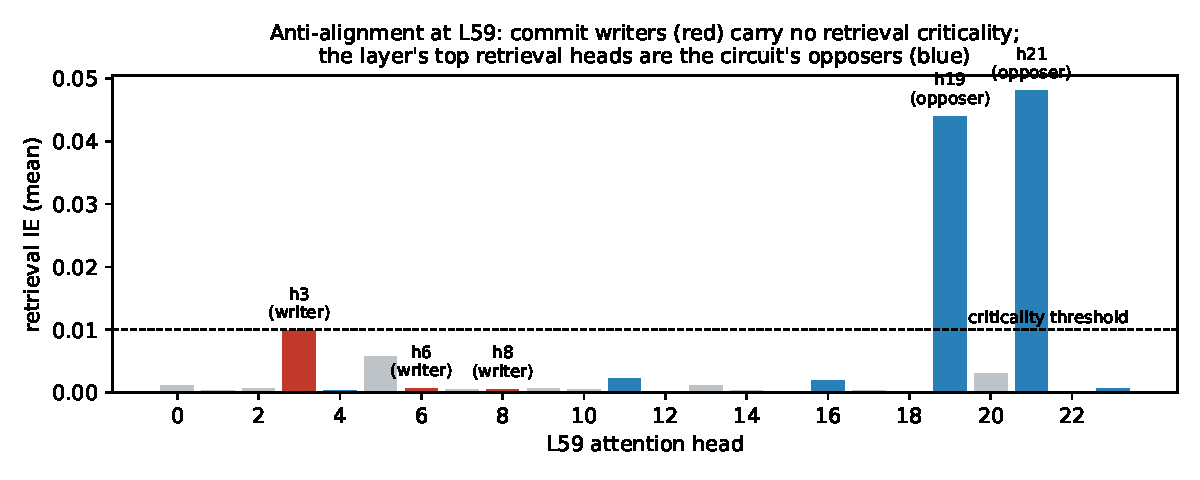
\includegraphics[width=0.95\linewidth]{figures/fig1_antialign_L59.pdf}
\caption{Retrieval importance (receiver IE, mean over 12 pairs) for all 24 heads of L59. The commit
writers (red) sit at the floor; the layer's strongest retrieval heads (blue) are the commitment circuit's
opposers.}\label{fig:antialign}
\end{figure}

Within L59 (Figure~\ref{fig:antialign}), retrieval-criticality and commitment-writing are \emph{anti-aligned}. The selection keeps 1 of
3 writers and 2 of 6 opposers: the push--pull circuit is shredded asymmetrically. This recurses a lesson
from the circuit's discovery one level up: there, geometric write magnitude misled about causal commit
(the largest writer was an opposer); here, \emph{causal capability-criticality} misleads about
\emph{safety-criticality}. A criterion being causal is not enough --- it is causal \emph{for its
capability set}.

\section{Stage 2: commitment collapses; the capability probe cannot notice}\label{sec:stage2}

Pre-registration note: the pre-registered primary scope (L59-only ablation) returned \emph{null} --- every
single-layer condition, including ablating the writers alone, is behaviorally silent ($\leq$2 flips):
natural commitment is redundant across the late band, mirroring the depth-distributed brake locus of
\citet{vicentino2026brake}. The band-scope result below is the pre-declared secondary condition, and we
label it exploratory relative to the pre-registration.

Ablating the 74 capability-non-retained heads of the late band (L51--63) under the criterion's keep-set:

\begin{table}[h]\centering\small
\resizebox{\columnwidth}{!}{%
\begin{tabular}{lccccc}
\toprule
condition & NIAH & $P(\text{edit})$@edit & emit@edit & emit@bash & McNemar vs base \\
\midrule
base & ceiling & 0.474 & 0.483 & 0.233 & --- \\
single-layer conditions ($\times$5) & ceiling & 0.44--0.49 & 0.45--0.48 & 0.23 & all n.s. \\
\textbf{drop non-retained, band (74h)} & ceiling & \textbf{0.167} & \textbf{0.183} & 0.183 & \textbf{18/0, $p{=}7.6{\times}10^{-6}$} \\
\bottomrule
\end{tabular}}
\caption{The two-sided audit. Task-appropriate commitment collapses --- the edit/bash differential
disappears ($0.25\to0.00$), with monotonic one-directional flips concentrated at edit points --- while
the NIAH readout never moves.}
\end{table}

\begin{figure}[t]\centering
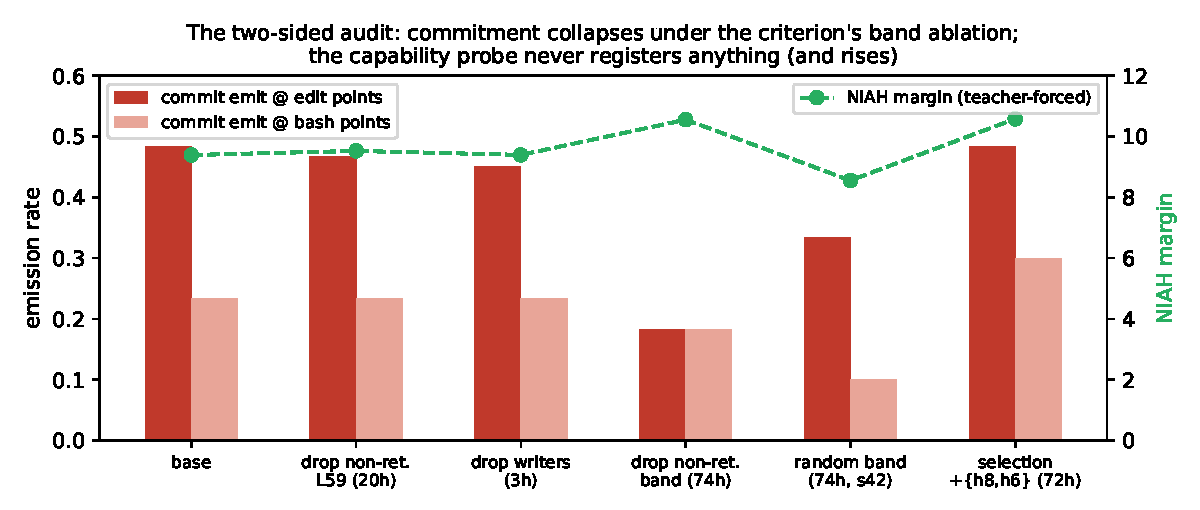
\includegraphics[width=0.95\linewidth]{figures/fig2_twosided.pdf}
\caption{The two-sided audit across conditions: commitment emission (bars, left axis) versus the
teacher-forced NIAH margin (green, right axis). Only the band-scope ablation of the criterion's
non-retained heads collapses commitment --- and the capability probe's margin \emph{rises}.}
\label{fig:twosided}
\end{figure}

\textbf{The capability side is untested, not ``passed'' --- and that is itself the finding
(Figure~\ref{fig:twosided}).} The
pre-registered positive control failed: ablating the retained retrieval heads at L59 did not hurt NIAH
(margin 9.29 vs base 9.39), and under the heaviest ablation the teacher-forced margin \emph{rises} (10.56).
An instrument whose margin increases when 74 heads are removed has no sensitivity at this difficulty (4K,
7-digit needle); its pass carries no information about capability preservation. We therefore claim only:
\emph{the capability probes that define the criterion are blind to the commitment collapse}. This sharpens
the audit thesis --- the criterion's own metric cannot see the damage --- while honestly conceding that
capability preservation itself was not measurable with our probe.

\section{Stages 3--4: controls}\label{sec:stage34}

\textbf{Worse than all five random selections.} Both arms keep exactly 22 late-band heads. Five random
draws (seeds 42--46) yield commitment $0.22$--$0.45$ (mean $0.33$); the capability-guided set yields
$0.183$, below all five (paired per-draw tests significant for 3/5; e.g.\ 10/1, $p{=}0.012$). The
membership pattern explains the mechanism: even a draw that drops \emph{all three} writers stays at 0.38
--- random keep-sets preserve commitment through other redundant band heads. The retrieval-only keep-set
is the \emph{least} commitment-redundant subset of its size; that, not writer membership alone, is why the
capability criterion is worst.

\begin{figure}[t]\centering
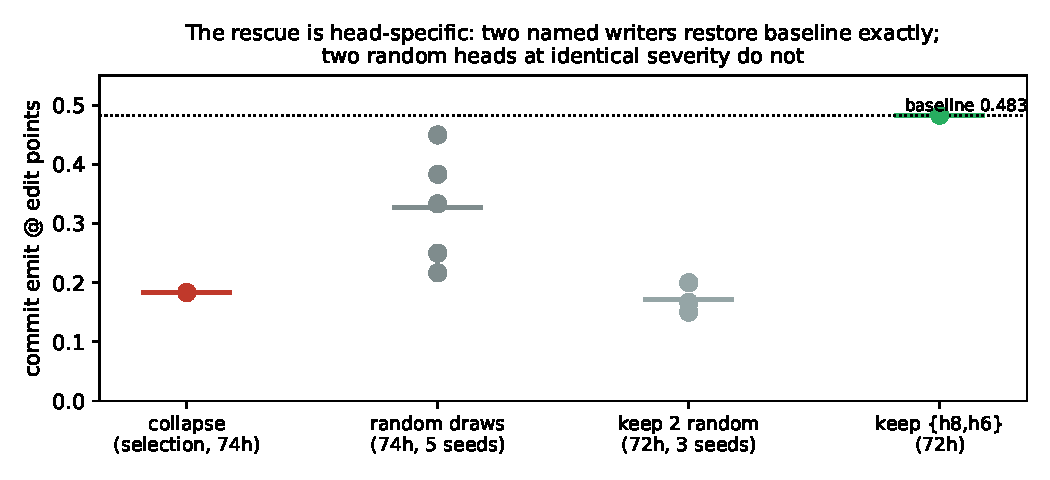
\includegraphics[width=0.85\linewidth]{figures/fig3_rescue.pdf}
\caption{Commitment at edit points by condition group (dots = runs, bars = means). The capability-guided
keep-set sits below all five random draws; restoring the two named writers --- and only them --- returns
exactly to baseline.}\label{fig:rescue}
\end{figure}

\textbf{The two-head rescue is head-specific (Figure~\ref{fig:rescue}).} Keeping the two named writers \{h8,h6\} while ablating the
other 72 heads restores commitment exactly (emit 0.483; $P(\text{edit})$ 0.487; \textbf{zero} per-point
flips vs base). Keeping two \emph{random} non-writer heads at identical severity leaves it collapsed
(0.150/0.167/0.200 across three seeds, mean 0.172; paired keep-writers vs keep-2-random: 17/0,
$p{=}1.5{\times}10^{-5}$). A residual over-commit trend at bash points (+4 flips, n.s.) is consistent with
the opposers remaining converted: the push returns without its pull. Jointly: \textbf{\{h8,h6\} ---
exactly the heads the criterion scores $\kappa{=}0$ --- are sufficient to carry task-appropriate
commitment once the band's redundancy is stripped, and their preservation costs 0.5\% of the FA-head
budget.} The constructive implication is a \emph{safety term} in the selection objective (a commitment
probe added to $C$), not a post-hoc whitelist: the criterion could have found these heads only by
measuring the behavior.

\section{Limitations}\label{sec:limitations}

(1) Mean-ablation upper-bounds pre-distillation damage; HydraHead's pipeline distills after conversion and
could recover the behavior --- we audit the \emph{selection criterion}, not the end-to-end recipe, and make
no claim that HydraHead-the-system is unsafe (different base model and scale).
(2) The capability probe lacked sensitivity (failed positive control); ``capability preserved'' is
untested. A harder long-context probe is future work.
(3) The global head ranking is unstable ($\rho{=}0.46$, zero-inflated); only named-head verdicts are
established.
(4) The pre-registered primary scope was null; the band-scope result is a labeled secondary.
(5) Emission applies ablation at prefill only (KV caching); $P(\text{edit})$ is the clean readout and
agrees.
(6) One model, one behavior family, $n{=}60$/side, uncorrected multiple comparisons (the headline
$p{=}7.6{\times}10^{-6}$ survives any correction; secondary $p{\approx}0.02$ results do not).
(7) Expansion samples share the probe template (same keys/filler); they double samples, not probe
diversity. Receivers-only IE (senders deferred).

\section{Conclusion}

Interpretability located a sparse, causal commitment circuit in an agentic model; a state-of-the-art
capability-guided efficiency criterion, applied to the same model, cannot see that circuit at all ---
scores it exactly zero --- and its keep-set collapses the agent's task-appropriate commitment more
thoroughly than chance would, while the criterion's own benchmarks register nothing. Two named heads,
identifiable only by causal circuit analysis, restore the behavior at negligible budget. The program this
extends is \emph{interpretability as audit}: not defending a model against adversaries, and now not only
auditing a fixed model's claims, but auditing the \emph{transformations} we apply to models ---
instantiating, against a concrete SOTA efficiency method, an audit agenda so far articulated only in
principle \citep{aigi2026agenda,makemi2026}. The mechanism-level moral is not new --- capability-aware
criteria concentrating damage on the unmeasured is known at weight granularity \citep{wei2024brittleness}
--- but the object-level facts are: a criterion, however causal, cannot see what it does not measure,
and neither can its benchmarks.

\paragraph{Reproducibility.} All numbers recompute from the public ledger
(\texttt{results/hydra\_audit\_ie.json}, HF \texttt{swebench-phase6-verdict-circuit}) via
\texttt{scripts/eval\_hydra\_audit.py} (59/59 checks); pre-registration, results log, and code in
\texttt{openinterp-swebench-harness}. under 6 GPU-hours on a single Colab G4 (block-time sum from run logs), across $\sim$15
short-lived VM incarnations over two days, zero data loss via per-stage checkpointing.

\begin{thebibliography}{99}
\sloppy
\bibitem[Tan et al.(2026)]{tan2026hydrahead} Z.~Tan, W.~Chen, J.~Shen, Y.~Liu, X.~Shen, Y.~Wu, J.~Ye.
HydraHead: From Head-Level Functional Heterogeneity to Specialized Attention Hybridization.
\emph{arXiv:2606.20097}, 2026.
\bibitem[Du et al.(2025)]{du2025rlkv} W.~Du et al. Which Heads Matter for Reasoning? RL-Guided KV Cache
Compression. \emph{arXiv:2510.08525}, 2025.
\bibitem[Wei et al.(2024)]{wei2024brittleness} B.~Wei et al. Assessing the Brittleness of Safety Alignment
via Pruning and Low-Rank Modifications. \emph{ICML}, 2024. arXiv:2402.05162.
\bibitem[Zhou et al.(2024)]{zhou2024safetyheads} Z.~Zhou et al. On the Role of Attention Heads in Large
Language Model Safety. \emph{ICLR}, 2025. arXiv:2410.13708.
\bibitem[Patel et al.(2025)]{patel2025aapp} D.~Patel et al. Alignment-Constrained Dynamic Pruning for LLMs:
Identifying and Preserving Alignment-Critical Circuits. \emph{arXiv:2511.07482}, 2025.
\bibitem[Dong et al.(2025)]{dong2025acbench} P.~Dong et al. Can Compressed LLMs Truly Act? An Empirical
Evaluation of Agentic Capabilities in LLM Compression. \emph{arXiv:2505.19433}, 2025.
\bibitem[Chen et al.(2025)]{chen2025qresafe} K.~Chen et al. Q-resafe: Assessing Safety Risks and
Quantization-aware Safety Patching for Quantized Large Language Models. \emph{ICML}, 2025.
arXiv:2506.20251.
\bibitem[Jahan et al.(2025)]{jahan2025distillation} S.~Jahan et al. Black-Box Behavioral Distillation
Breaks Safety Alignment in Medical LLMs. \emph{arXiv:2512.09403}, 2025.
\bibitem[Xiao et al.(2024)]{xiao2024duo} G.~Xiao et al. DuoAttention: Efficient Long-Context LLM Inference
with Retrieval and Streaming Heads. \emph{ICLR}, 2025. arXiv:2410.10819.
\bibitem[Tang et al.(2024)]{tang2024razor} H.~Tang et al. RazorAttention: Efficient KV Cache Compression
Through Retrieval Heads. \emph{arXiv:2407.15891}, 2024.
\bibitem[Chhabra et al.(2025)]{yao2025refusalcompressed} V.~K.~Chhabra et al. Towards Understanding and
Improving Refusal in Compressed Models via Mechanistic Interpretability. \emph{arXiv:2504.04215}, 2025.
\bibitem[Ni et al.(2026)]{anchorskv2026} N.~Ni et al. AnchorKV: Safety-Aware KV Cache Compression via
Soft Penalty with a Refusal Anchor. \emph{arXiv:2606.17872}, 2026.
\bibitem[Benfeghoul et al.(2025)]{yang2025untangling} M.~Benfeghoul et al. Untangling Component Imbalance
in Hybrid Linear Attention Conversion Methods. \emph{arXiv:2510.05901}, 2025.
\bibitem[Gupta et al.(2026)]{cgc2026} R.~Gupta et al. Capability-Guided Compression: Toward
Interpretability-Aware Budget Allocation for Large Language Models. \emph{arXiv:2603.16440}, 2026.
\bibitem[Lan et al.(2026)]{makemi2026} M.~Lan et al. Make Mechanistic Interpretability Auditable: A Call
to Develop Guidelines via Continuous Collaborative Reviewing. \emph{arXiv:2606.00033}, ACL 2026.
\bibitem[Oxford Martin AIGI(2026)]{aigi2026agenda} Automated Interpretability-Driven Model Auditing and
Control: A Research Agenda. Oxford Martin AIGI, January 2026.
\url{https://aigi.ox.ac.uk/publications/automated-interpretability-driven-model-auditing-and-control-a-research-agenda/}
\bibitem[Wu et al.(2024)]{wu2024retrieval} W.~Wu et al. Retrieval Head Mechanistically Explains
Long-Context Factuality. \emph{ICLR}, 2025. arXiv:2404.15574.
\bibitem[Vicentino(2026a)]{vicentino2026lever} C.~Vicentino. The Lever Is Late: the Knowledge--Action Gap
in a Long-Horizon Agent Is a Layer Gap. Zenodo, 2026. doi:10.5281/zenodo.20534218.
\bibitem[Vicentino(2026b)]{vicentino2026brake} C.~Vicentino. The Commitment Lever Generalizes --- and
Brakes. Zenodo, 2026. doi:10.5281/zenodo.20634837.
\bibitem[Vicentino(2026c)]{vicentino2026located} C.~Vicentino. Located, Not Secured: What Interpretability
Buys for Agent Safety. Zenodo, 2026. doi:10.5281/zenodo.20764857.
\end{thebibliography}

\end{document}
